% $Header: /home/vedranm/bitbucket/beamer/solutions/generic-talks/generic-ornate-15min-45min.en.tex,v 90e850259b8b 2007/0\frac{1}{2}8 20:48:30 tantau $
\documentclass{beamer}
%\documentclass[handout]{beamer}
\usefonttheme[onlymath]{serif}
% This file is a solution template for:
\usepackage{algcompatible}
\usepackage{algpseudocode}
\usepackage{multicol}
\usepackage{animate}
% - Giving a talk on some subject.
% - The talk is between 15min and 45min long.
% - Style is ornate.
% Copyright 2004 by Till Tantau <tantau@users.sourceforge.net>.
%
% In principle, this file can be redistributed and/or modified under
% the terms of the GNU Public License, version 2.
%
% However, this file is supposed to be a template to be modified
% for your own needs. For this reason, if you use this file as a
% template and not specifically distribute it as part of a another
% package/program, I grant the extra permission to freely copy and
% modify this file as you see fit and even to delete this copyright
% notice. 

\mode<presentation>
{
  \usetheme{Warsaw}
  % or ...

  \setbeamercovered{transparent}
  % or whatever (possibly just delete it)
}
\setbeamertemplate{navigation symbols}{} 

\usepackage[english]{babel}
% or whatever

\usepackage[latin1]{inputenc}
% or whatever
\useoutertheme{default}

\usepackage{times}
\usepackage[T1]{fontenc}
% Or whatever. Note that the encoding and the font should match. If T1
% does not look nice, try deleting the line with the fontenc.
\newcommand{\beforeverb}{\footnotesize}
\newcommand{\afterverb}{\normalsize}

\title[Boundary-Value Problems for Ordinary
Differential Equations] % (optional, use only with long paper titles)
{Lecture 13}

\subtitle
{Boundary-Value Problems for Ordinary
Differential Equations} % (optional)

\author[Ying-Jer Kao] % (optional, use only with lots of authors)
{Ying-Jer Kao}
% - Use the \inst{?} command only if the authors have different
%   affiliation.

\institute[National Taiwan University] % (optional, but mostly needed)
{
  Department of Physics\\
 National Taiwan University
  }
% - Use the \inst command only if there are several affiliations.
% - Keep it simple, no one is interested in your street address.

\date[Numerical Analysis and Programming] % (optional)
{\today}

\subject{Talks}
% This is only inserted into the PDF information catalog. Can be left
% out. 



% If you have a file called "university-logo-filename.xxx", where xxx
% is a graphic format that can be processed by latex or pdflatex,
% resp., then you can add a logo as follows:

% \pgfdeclareimage[height=0.5cm]{university-logo}{university-logo-filename}
% \logo{\pgfuseimage{university-logo}}



% Delete this, if you do not want the table of contents to pop up at
% the beginning of each subsection:
%\AtBeginSubsection[]
%{
%  \begin{frame}<beamer>{Outline}
%    \tableofcontents[currentsection,currentsubsection]
%  \end{frame}
%}


% If you wish to uncover everything in a step-wise fashion, uncomment
% the following command: 

%\beamerdefaultoverlayspecification{<+->}


\begin{document}

\begin{frame}
  \titlepage
\end{frame}

\begin{frame}{Outline}
  \tableofcontents
  % You might wish to add the option [pausesections]
\end{frame}


% Since this a solution template for a generic talk, very little can
% be said about how it should be structured. However, the talk length
% of between 15min and 45min and the theme suggest that you stick to
% the following rules:  

% - Exactly two or three sections (other than the summary).
% - At *most* three subsections per section.
% - Talk about 30s to 2min per frame. So there should be between about
%   15 and 30 frames, all told.
\section[Introduction]{Introduction}
\begin{frame}{Introduction}
\begin{itemize}
    \item The boundary-value problem for ordinary differential equations is to find a solution 
    to the differential equation that satisfies certain specified conditions at the 
    endpoints of the interval.
    \[
    y'' = f(x, y, y'), \quad y(a) = \alpha, \quad y(b) = \beta
    \]
    \item The boundary-value problem is more difficult than the initial-value problem.
    \item In the initial-value problem, we can use the initial conditions to determine 
    the constants of integration.
    \item In the boundary-value problem, we have to solve the differential equation and satisfies 
    the boundary conditions simultaneously.
\end{itemize}
\end{frame}
\begin{frame}{Introduction: Shooting Method}

    \begin{itemize}
        \item One way to overcome the lack of starting conditions is to guess the missing values.
        \item The resulting solution is unlikely to satisfy boundary conditions at the other end, but:
        \begin{itemize}
            \item By inspecting the discrepancy, one can estimate changes to make to the initial conditions.
            \item This iterative procedure is known as the \textit{shooting method}.
        \end{itemize}
        \item The shooting method name is derived from analogy with target shooting:
        \begin{itemize}
            \item Take a shot and observe where it hits the target.
            \item Correct the aim and shoot again.
        \end{itemize}

    \end{itemize}
\end{frame}
\begin{frame}{Introduction: Finite Difference Method}
    \begin{itemize}
        \item Another method for solving two-point boundary value problems is the \textit{finite difference method}:
        \begin{itemize}
            \item Differential equations are approximated by finite differences at evenly spaced mesh points.
            \item This transforms the differential equation into a set of simultaneous algebraic equations.
        \end{itemize}   
    \end{itemize}
\end{frame}

\begin{frame}{Shooting Method}
    \begin{itemize}
        \item Take the boundary-value problem
        \[
    y'' = f(x, y, y'), \quad y(a) = \alpha, \quad y(b) = \beta
    \]
    \item The shooting method is to convert the boundary-value problem into an initial-value problem.
    \item To solve an initial-value problem, we need to specify the initial conditions, $y(a)=\alpha$ and $y'(a)$.
    \item We guess $y'(a)$ and solve the initial-value problem.
    \item If $y(b)$ is close to $\beta$, we are done.
    \item Otherwise, we adjust $y'(a)$ and solve the initial-value problem again until $y(b)$ is close to $\beta$.
    \end{itemize}
\end{frame}
\begin{frame}{Shooting Method}
    \centerline{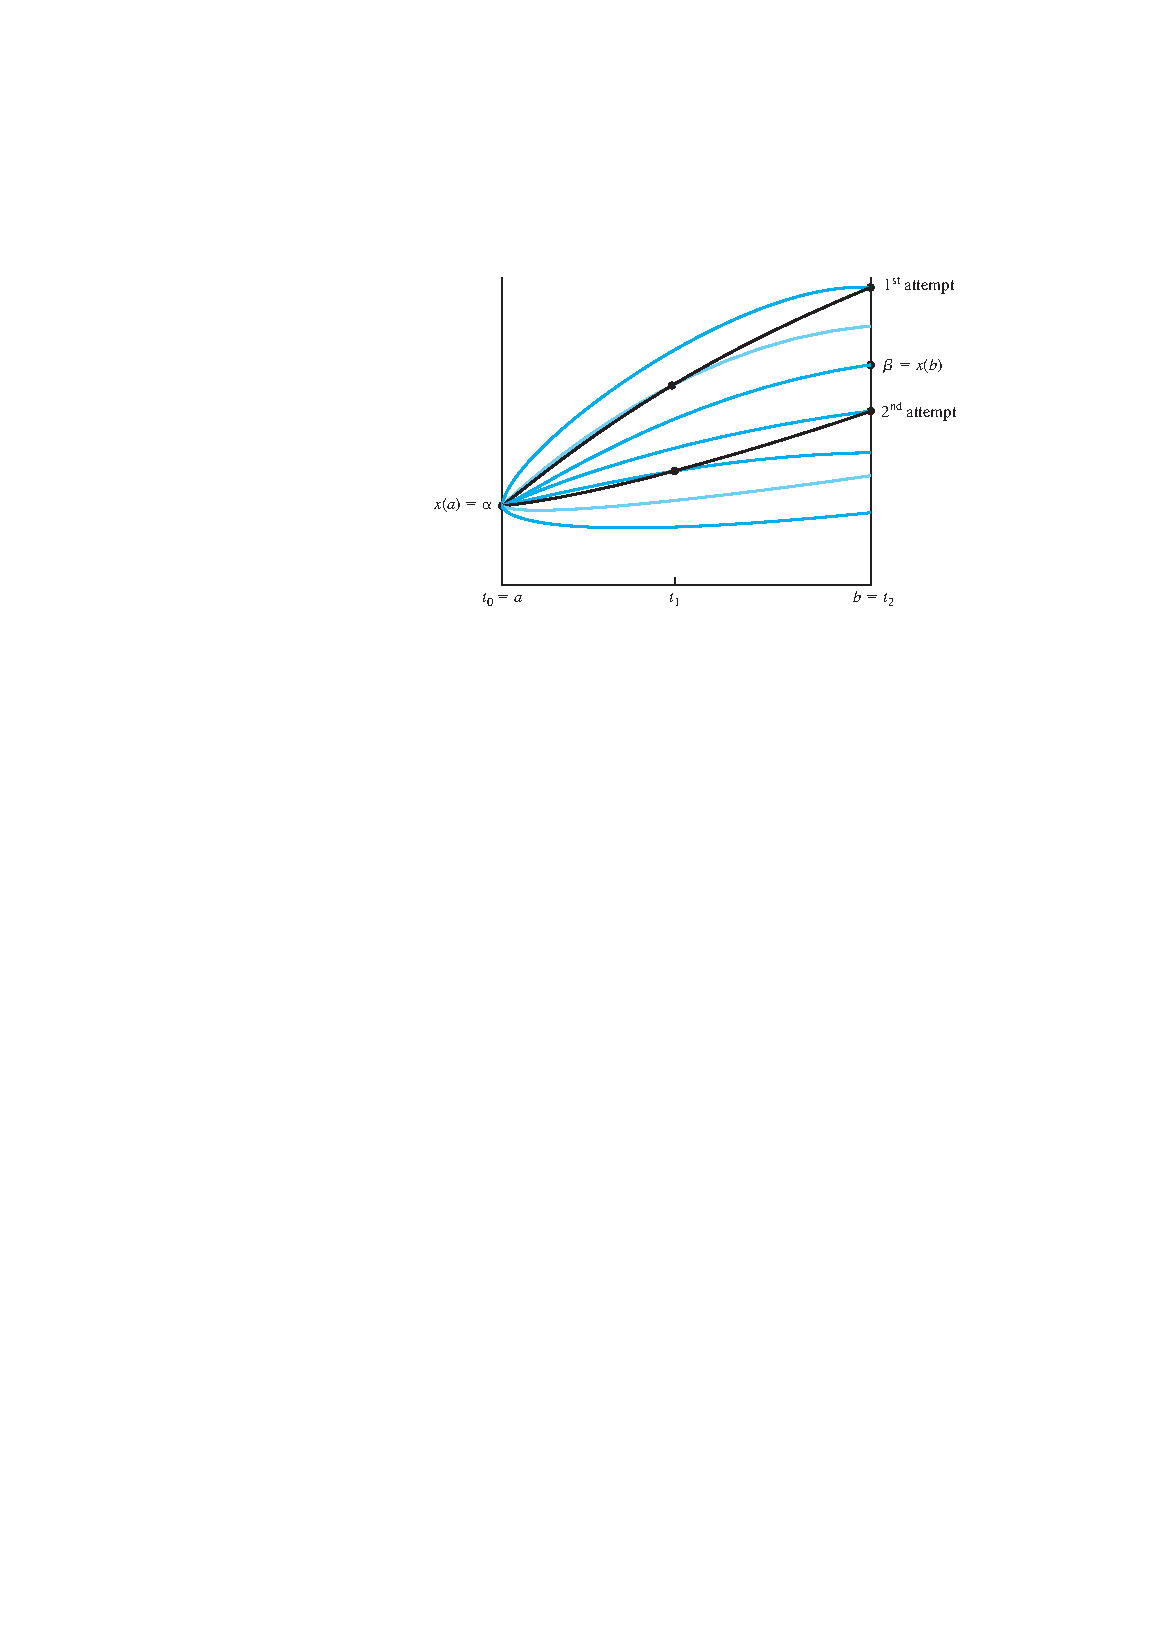
\includegraphics[width=0.95\textwidth]{ShootingMethod.pdf}}

\end{frame}
\begin{frame}{Adjusting the Initial Conditions}
    \begin{itemize}
        \item Suppose we have a guess of $y'(a)$, we can solve the initial-value problem to get $y(b)$.
        \item If $y(b)$ is not close to $\beta$, we need to adjust $y'(a)$.
        \item We can use the secant method to adjust $y'(a)$.
        \[
        y'(a) = y'(a) - \frac{y(b) - \beta}{y(b) - y(b)_{\textrm{old}}} (y'(a) - y'(a)_{\textrm{old}})
        \]
        \item We repeat the process until $y(b)$ is close to $\beta$.
    \end{itemize}
\end{frame}
\begin{frame}{Example: Shooting Method}
    \begin{itemize}
        \item Consider the boundary-value problem
        \[
        y'' = -y, \quad y(0) = 0, \quad y(\pi/2) = 1
        \]
        \item We can convert the boundary-value problem into an initial-value problem by guessing $y'(0)$.
        \item We can use the secant method to adjust $y'(0)$.
    \end{itemize}

\end{frame}
\begin{frame}{Higer-Order Differential Equations}
    \begin{itemize}
        \item Consider the fourth-order differential equation with boundary conditions
        \[
        y^{(4)} = f(x, y, y', \ldots, y^{(n-1)}), \quad y(a)=\alpha_1 \quad y^{\prime \prime}(a)=\alpha_2
         \quad y(b)=\beta_1 \quad y^{\prime \prime}(b)=\beta_2 
        \]
        \item We need four initial conditions to solve the differential equation, but have only two.
        \item We guess the missing initial conditions as $u_1$ and $u_2$.
        \[
            y(a)=\alpha_1 \quad y^{\prime}(a)=u_1 \quad y^{\prime \prime}(a)=\alpha_2 \quad y^{\prime \prime \prime}(a)=u_2
        \]
        \item The computated boundary values at $x=b$ depends on $u_1$ and $u_2$, and we need to solve the following system of equations
        \[
            y(b)=\theta_1\left(u_1, u_2\right)=\beta_1 \quad y^{\prime \prime}(b)=\theta_2\left(u_1, u_2\right)=\beta_2
        \]
    \end{itemize}
\end{frame}
\begin{frame}{Shooting Method: Summary}
    \begin{itemize}
        \item The shooting method is simple but time consuming.
        \item The shooting method does not always converge.
        \item The shooting method is not efficient for large systems.
        \item In practice, we start with a large step size $h$ such that the boundary
        condition is satisfied. We then reduce the step size to get a more accurate solution.

    \end{itemize}
\end{frame}
\begin{frame}{Finite Difference Method}
    \begin{itemize}
        \item The finite difference method is a discretizatin mehtod to solve boundary-value problems.
        \item The finite difference method is to approximate the differential equation by finite differences.
        \item We can then solve the resulting algebraic equations.
        \item The finite difference method is more efficient than the shooting method for large systems.
    \end{itemize}

\end{frame}
\begin{frame}{Finite Difference Method}
    \begin{itemize}
        \item Consider the boundary-value problem
        \[
        y'' = f(x, y, y'), \quad y(a) = \alpha, \quad y(b) = \beta
        \]
        \item We can approximate the second derivative by the central difference formula
        \[
        y''(x) \approx \frac{y(x+h) - 2y(x) + y(x-h)}{h^2},
        \]
        and the first derivative is 
        \[
        y'(x) \approx \frac{y(x+h) - y(x-h)}{2h},
        \]
        where $h=(b-a)/N$. 
        
    \end{itemize}
\end{frame}
\begin{frame}{Finite Difference Method}
\begin{itemize}
    \item We can approximate the differential equation by finite differences
    \item Denote $y_i=y(x_i)$, where $x_i=a+ih$.
    \item The differential equation becomes 
    \[
    \frac{y_{i+1} - 2y_i + y_{i-1}}{h^2} = f(x_i, y_i, (y_{i+1} - y_{i-1})/(2h)), \quad i=1, 2, \ldots, N-1.
    \]
   \item This is uaually a nonlinear systems of equations in the $N-1$ unknowns $y_1, y_2, \ldots, y_{N-1}$.
\end{itemize}
\end{frame}
\begin{frame}{Linear Case}
    \begin{itemize}
        \item If $f(x,y,y')=u(x)+v(x)y+w(x)y'$, the differential equation is lieanr and the finite difference equation is linear.
        \item We have 
        \[
            \frac{y_{i+1} - 2y_i + y_{i-1}}{h^2} = u(x)+v(x)y+\frac{y_{i+1} - y_{i-1}}{2h}w(x),
        \]
        or equvalently
        \[
            -\left(1+\frac{h}{2} w_i\right)
             y_{i-1}+\left(2+h^2 v_i\right) y_i-\left(1-\frac{h}{2} w_i\right) y_{i+1}=-h^2 u_i,
        \]
        where $u_i=u(x_i)$, $v_i=v(x_i)$, and $w_i=w(x_i)$.
    \end{itemize}
\end{frame}
\begin{frame}{Linear Case (Cont.)}
    \begin{itemize}
        \item Denote
     $a_i = -\left(1+\frac{h}{2} w_i\right)$,$ b_i = \left(2+h^2 v_i\right)$,
     $c_i = -\left(1-\frac{h}{2} w_i\right)$, $ d_i = -h^2 u_i$.
       \item The finite difference equation is 
     \[
        a_i y_{i-1} + b_i y_i + c_i y_{i+1} = d_i, \quad i=1, 2, \ldots, N-1.
     \]
     or in the matrix form
        \[
        \begin{pmatrix}
            b_1 & c_1 & 0 & \cdots & 0 \\
            a_2 & b_2 & c_2 & \cdots & 0 \\
            0 & a_3 & b_3 & \cdots & 0 \\
            \vdots & \vdots & \vdots & \ddots & \vdots \\
            0 & 0 & 0 & \cdots & b_{N-1}
        \end{pmatrix} \begin{pmatrix}
            y_1 \\ y_2 \\ y_3\\\vdots \\ y_{N-1}  
        \end{pmatrix} = \begin{pmatrix}
            d_1-\alpha a_1 \\ d_2 \\d_3 \\ \vdots \\ d_{N-1}-\beta c_{N-1}
        \end{pmatrix},   
        \]
        where $y_0=y(a)=\alpha$ and $y_N=y(b)=\beta$ are used. 
    \end{itemize}

\end{frame}
\begin{frame}{Fourth-order Differential Equation}
    \begin{itemize}
        \item Consider the fourth-order differential equation 
        \[
        y^{(4)} = f(x, y, y', \ldots, y^{(n-1)}),  
        \]
        with boundary conditions $y(a)=y'(a)=y''(a)=y'''(a)=\alpha$ and $y(b)=y'(b)=y''(b)=y'''(b)=\beta$.
        \item The finite difference equation is
        \[
            \frac{y_{i-2}-4 y_{i-1}+6 y_i-4 y_{i+1}+y_{i+2}}{h^4}=f\left(x_i, y_i, \frac{y_{i-1}-2 y_i+y_{i+1}}{h^2}\right)
        \]

    \end{itemize}
\end{frame}

\begin{frame}
    \begin{itemize}
        \item The  equations near the boundaries are
        \beforeverb
        \begin{align*}
        \frac{y_{-2}-4y_{-1}+6y_0-4y_1+y_2}{h^4}&=f\left(x_0, y_0, \frac{y_{-1}-2 y_0+y_1}{h^2}\right)\\
        \frac{y_{-1}-4y_0+6y_1-4y_2+y_3}{h^4}&=f\left(x_1, y_1, \frac{y_0-2 y_1+y_2}{h^2}\right)\\
        \frac{y_{0}-4y_1+6y_2-4y_3+y_4}{h^4}&=f\left(x_2, y_2, \frac{y_1-2 y_2+y_3}{h^2}\right)\\
        \vdots\\
        \frac{y_{N-3}-4y_{N-2}+6y_{N-1}-4y_N+y_{N+1}}{h^4}&=f\left(x_{N-1}, y_{N-1}, \frac{y_{N-2}-2 y_{N-1}+y_N}{h^2}\right)\\
        \frac{y_{N-2}-4y_{N-1}+6y_N-4y_{N+1}+y_{N+2}}{h^4}&=f\left(x_N, y_N, \frac{y_{N-1}-2 y_N+y_{N+1}}{h^2}\right)
        \end{align*}
        \afterverb
        \item There are terms outside the domain of the problem, and can be fixed by the boundary conditions.
    \end{itemize}
\end{frame}
\begin{frame}
    \begin{tabular}{|r|l|}
        \hline Boundary cond. & Equivalent finite difference expression \\
        \hline$y(a)=\alpha$ & $y_0=\alpha$ \\
        $y^{\prime}(a)=\alpha$ & $y_{-1}=y_1-2 h \alpha$ \\
        $y^{\prime \prime}(a)=\alpha$ & $y_{-1}=2 y_0-y_1+h^2 \alpha$ \\
        $y^{\prime \prime \prime}(a)=\alpha$ & $y_{-2}=2 y_{-1}-2 y_1+y_2-2 h^3 \alpha$ \\
        \hline$y(b)=\beta$ & $y_m=\beta$ \\
        $y^{\prime}(b)=\beta$ & $y_{N+1}=y_{N-1}+2 h \beta$ \\
        $y^{\prime \prime}(b)=\beta$ & $y_{N+1}=2 y_m-y_{N-1}+h^2 \beta$ \\
        $y^{\prime \prime \prime}(b)=\beta$ & $y_{N+2}=2 y_{N+1}-2 y_{N-1}+y_{N-2}+2 h^3 \beta$ \\
        \hline
        \end{tabular}

        \begin{itemize}
            \item Notice that not all boundary conditions can be used to eliminate the terms outside the domain.
            \item  For example, $y(a)=\alpha_1$ and $y'''(a)=\alpha_2$ or $y'(a)=\alpha_1$ and $y''(a)=\alpha_2$, 
            we can not eliminate the terms outside the domain. 
        \end{itemize}
        
\end{frame}
\begin{frame}{Partial Differential Equations}
\begin{itemize}
    \item A partial differential equation (PDE) is an equation involving an unknown function of two or more variables and its partial derivatives.
    \item The general form of a PDE is
     \[
     F(x, y, z, u, u_x, u_y, u_z, u_{xx}, u_{xy}, u_{xz}, u_{yy}, u_{yz}, u_{zz}) = 0,
     \]
     where $u$ is the unknown function, and $u_x$, $u_y$, $u_z$, $u_{xx}$, $u_{xy}$, $u_{xz}$, $u_{yy}$, $u_{yz}$, $u_{zz}$ are the partial derivatives of $u$.
\item The order of a PDE is the order of the highest derivative in the equation.
\item PDEs can
lead to some of the most challenging of numerical problems. 

\end{itemize}
\end{frame}
\begin{frame}{Examples of PDEs}
    \begin{itemize}
            \item Heat equation $\frac{1}{k} \frac{\partial u}{\partial t}=\nabla^2 u$.
            \item Wave equation $\frac{1}{c^2} \frac{\partial^2 u}{\partial t^2}=\nabla^2 u$.

            \item Poisson equation $\nabla^2 u = f(x, y, z)$.
            \item Laplace equation $\nabla^2 u = 0$.
            \item Helmholtz equation $\nabla^2 u + k^2 u = 0$.
            \item Diffusion equation $\frac{\partial u}{\partial t} = D \nabla^2 u$.
            \item Navier-Stokes equation 
            \[
            \rho \left(\frac{\partial \mathbf{v}}{\partial t} + \mathbf{v} \cdot \nabla
             \mathbf{v}\right) = -\nabla p + \mu \nabla^2 \mathbf{v} + \mathbf{f}.
            \]
        \end{itemize}
\end{frame}
\begin{frame}{Types of PDEs:}

    \begin{itemize}
        \item Elliptic PDEs
        \[\nabla^2 u = f(x, y, z).
        \]
        
        \item Parabolic PDEs: 
        \[\frac{\partial u}{\partial t} = \nabla^2 u\]
        \item Hyperbolic PDEs\[\frac{\partial^2 u}{\partial t^2} = \nabla^2 u.\]
    \end{itemize}

\end{frame}
\begin{frame}{Types of Boundary Conditions}

    \begin{itemize}
     \item Dirichlet boundary condition: $$u(x, y) = g(x, y)$$.
    \item Neumann boundary condition: $$\frac{\partial u}{\partial n} = g(x, y)$$.
    \item Mixed boundary condition: $$\alpha u + \beta \frac{\partial u}{\partial n} = g(x, y)$$.
    \end{itemize}
\end{frame}
\begin{frame}{Parabolic PDE}
    \begin{itemize}
        \item Consider the heat equation
        \[
            \frac{\partial^2}{\partial x^2} u(x, t)  =\frac{\partial}{\partial t} u(x, t), \]
            where the boundary conditions are
            \[
            u(0, t)  =u(1, t)=0 \]
            and the initial condition is 
            \[ u(x, 0)  =\sin \pi x
            \]
        \item We can use the finite difference method to solve the heat equation.
    \end{itemize}

\end{frame}
\begin{frame}{Heated Rod}
\centerline{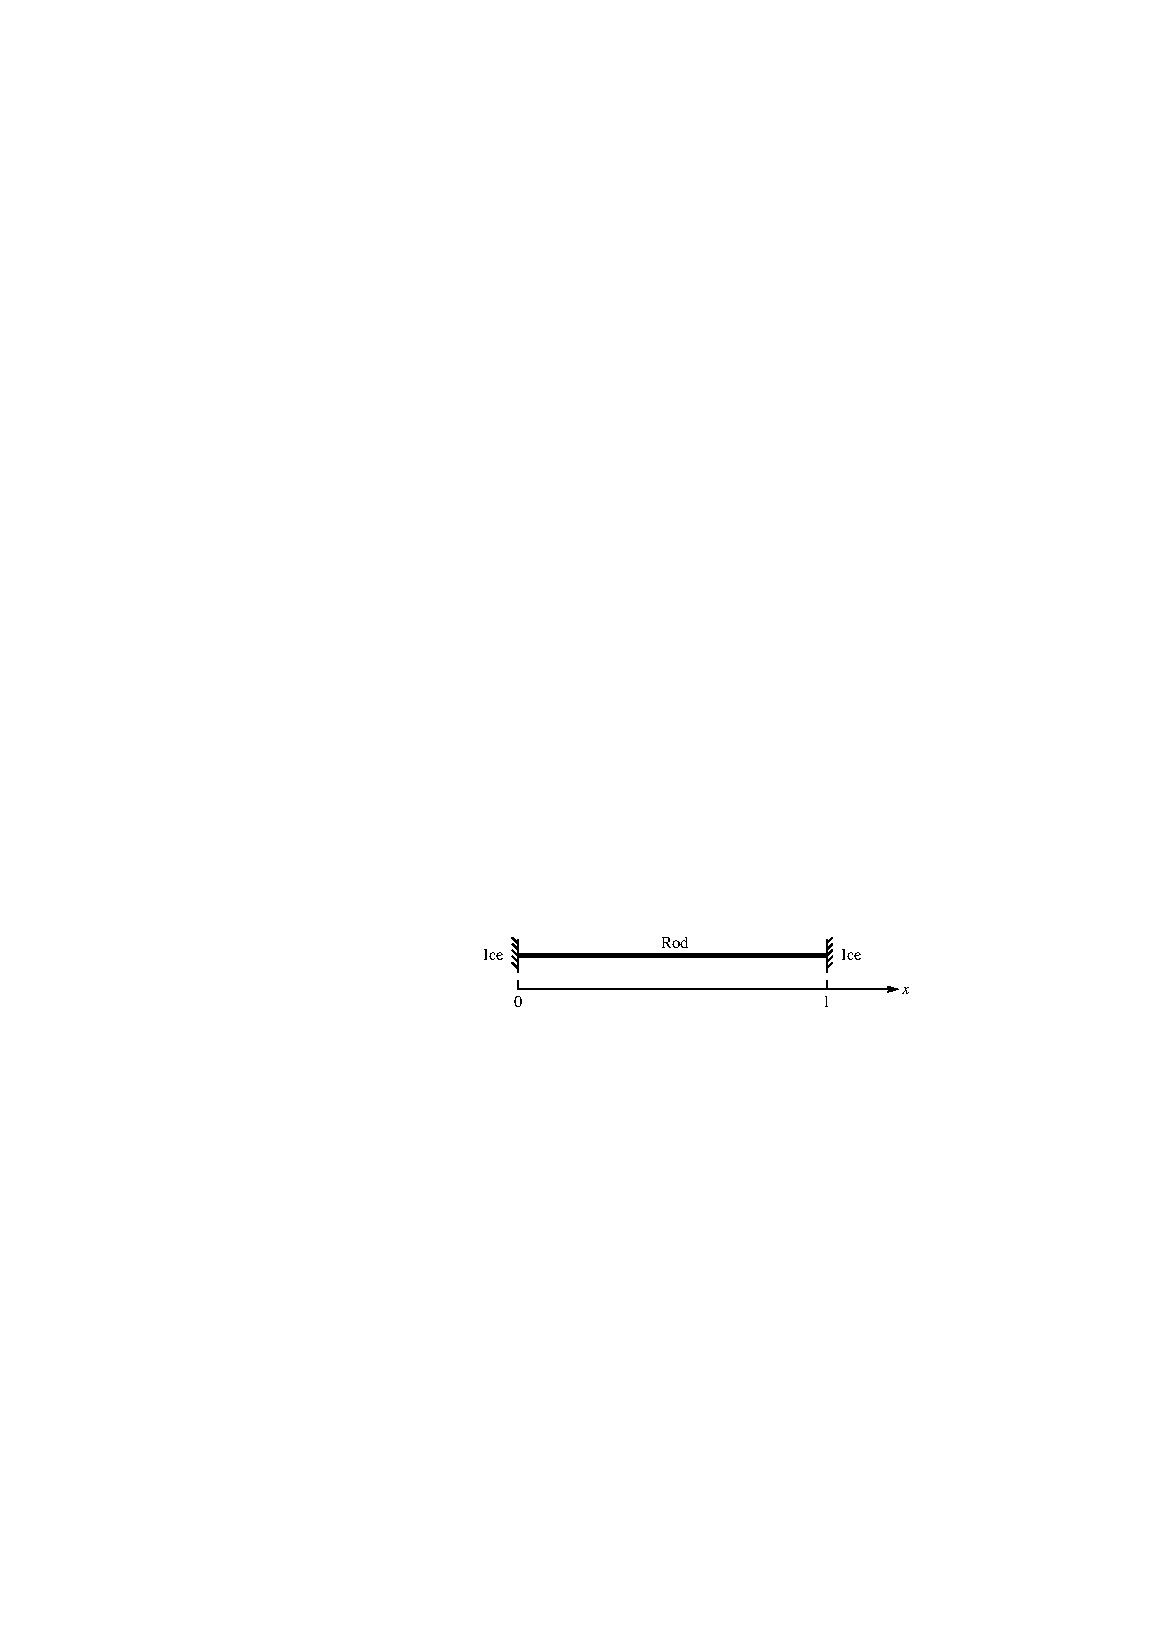
\includegraphics[width=0.6\textwidth]{HeatedRod.pdf}}
\begin{itemize}

    \item Approximating the first and second derivatives by finite differences, and consider different steps 
    $h$ and $k$ for $x$ and $t$, we have
    \[
    \frac{1}{h^2}[u(x+h, t)-2 u(x, t)+u(x-h, t)]=\frac{1}{k}[u(x, t+k)-u(x, t)]
    \]
    \item We advance the solution in time by solving the above equation.
\end{itemize}

\end{frame}
\begin{frame}{Heated Rod}
    \centerline{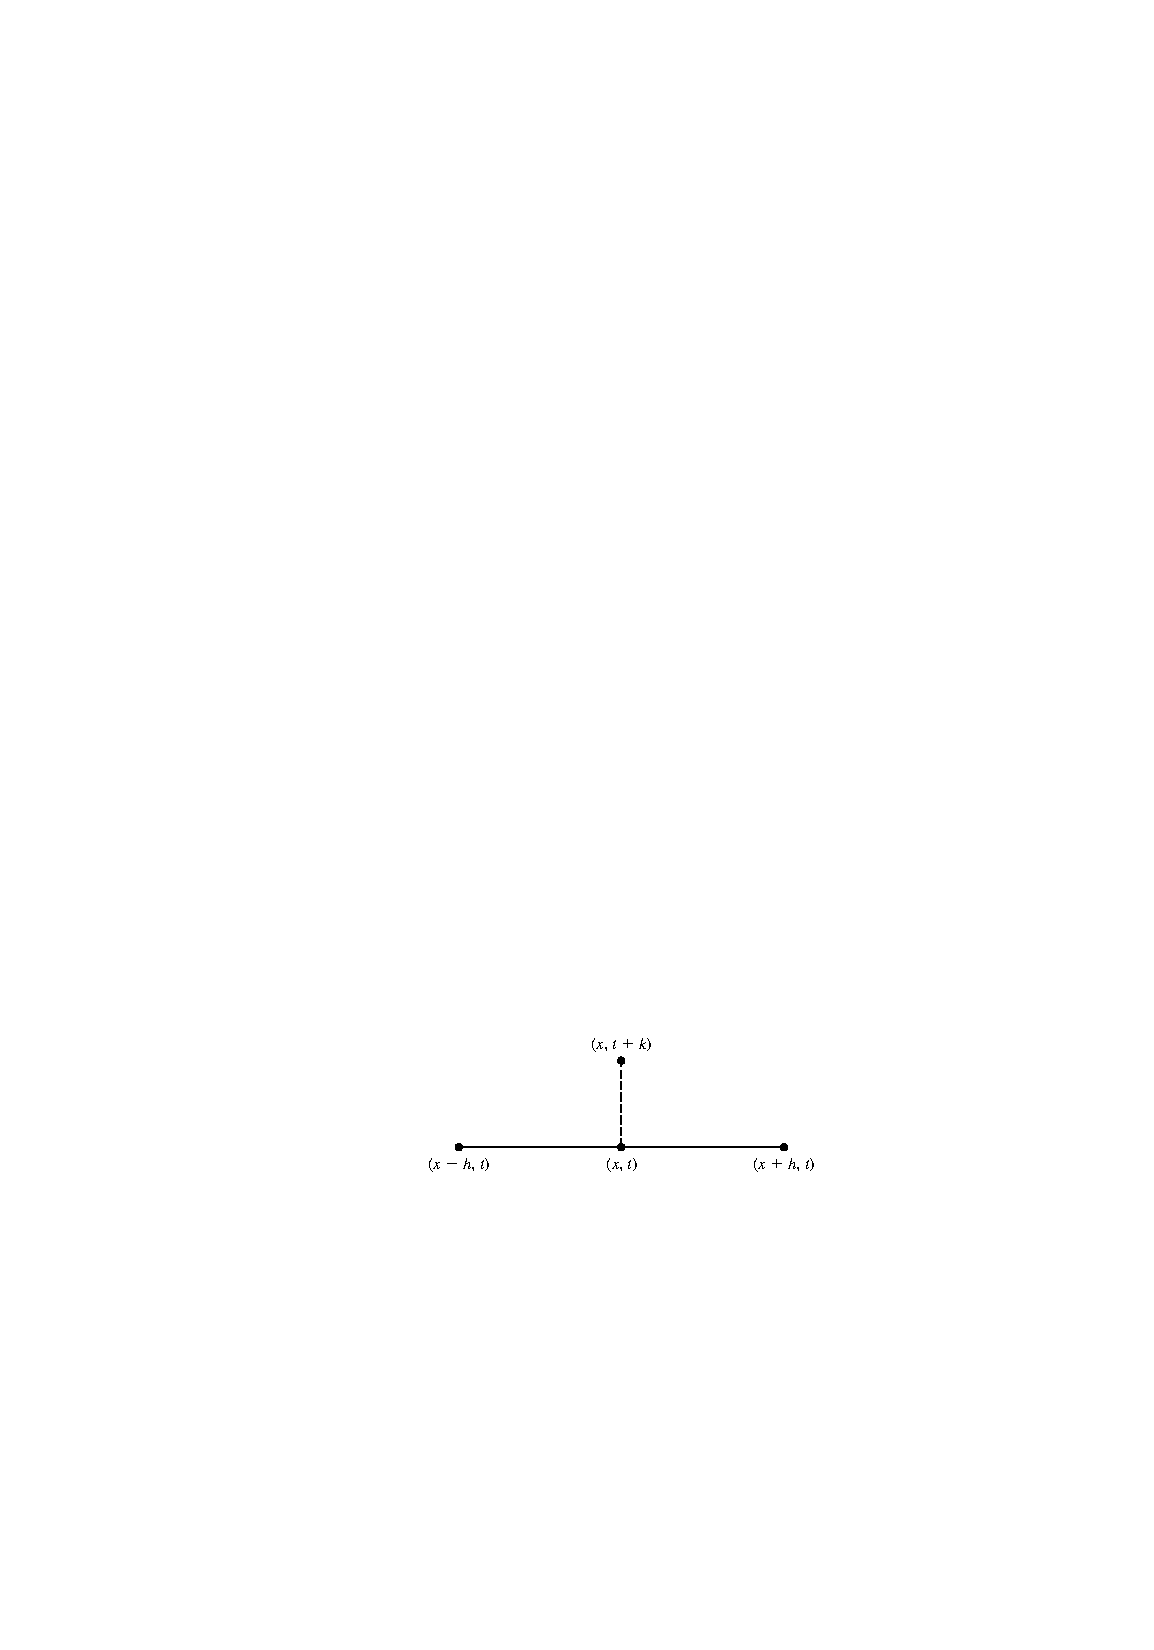
\includegraphics[width=0.6\textwidth]{HeatEqnExplicit.pdf}}
    \begin{itemize}
        \item Rewring the above equation, we have the explicit method,
        \[
        u(x, t+k)=\sigma u(x+h, t)+(1-2 \sigma) u(x, t)+\sigma u(x-h, t),
    \]
    where $\sigma=k/h^2$.
    \item If $u(x,t)$ is known, we can advance the solution to $t+\Delta t$.
    \end{itemize}

\end{frame}
\begin{frame}{Explicit Method:PseudoCode}
    \begin{algorithmic}
        \Procedure{HeatEquation}{$N, M$}
        \State $h \gets 1/N$
        \State $k \gets 1/M$
        \State $\sigma \gets k/h^2$
        \For{$i=1$ to $N-1$}
        \State $u[i] \gets \sin(\pi i h)$
        \EndFor
        \For{$j=1$ to $M$}
        \For{$i=1$ to $N-1$}
        \State $u[i] \gets \sigma u[i+1]+(1-2\sigma)u[i]+\sigma u[i-1]$
        \EndFor
        \EndFor
        \EndProcedure
    \end{algorithmic}
    
\end{frame}
\begin{frame}{Explicit Method: Stability}
    \begin{itemize}
        \item In the explicit method, approximate values
        of $u(x, t +k)$ are calculated explicitly in terms of $u(x, t)$.
        \item The explicit method is conditionally stable.
        \item The stability condition is $\sigma =\frac{k}{h^2}\leq 1/2$.
        \item Since $h$ must be rather small to represent the derivative accurately by the finite difference
        formula, the corresponding $k$ must be extremely small.
        \item For example, $h=0.01$ and $k=0.00005$ are typical values. This makes the method very inefficient.
    \end{itemize}
\end{frame}
\begin{frame}{Crank-Nicolson Method}
    \centerline{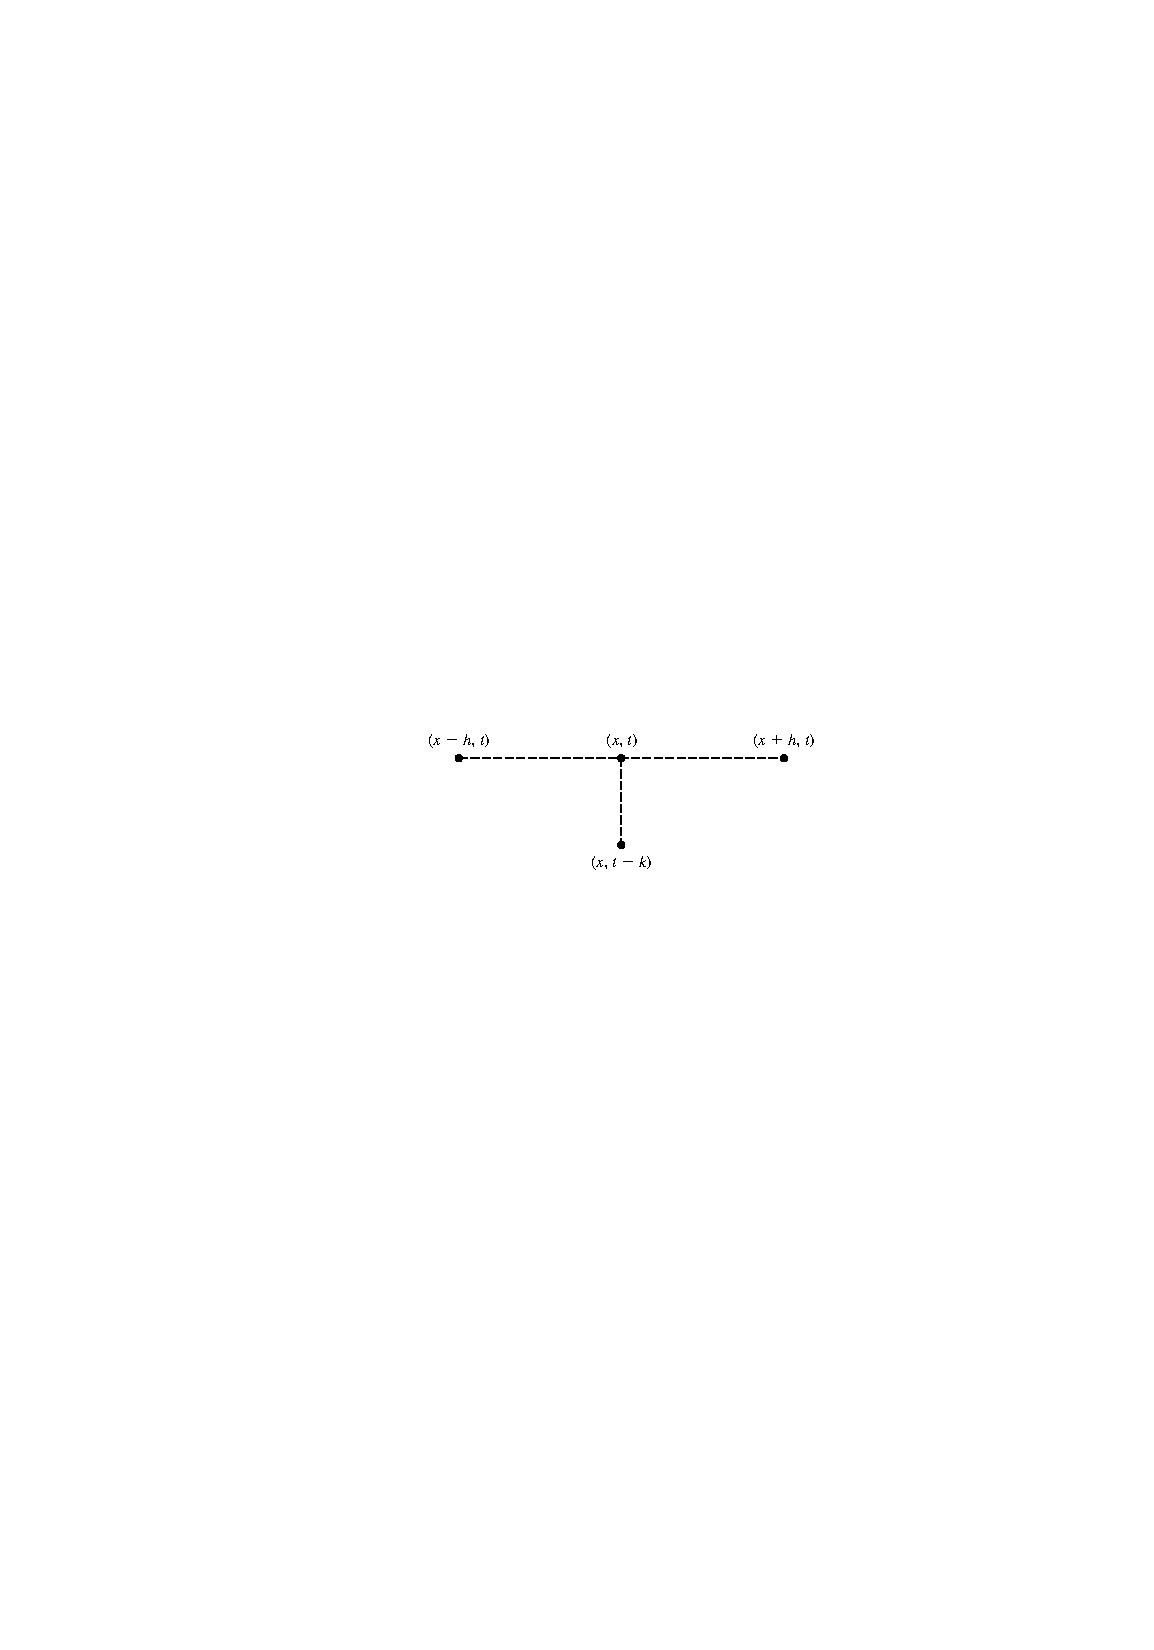
\includegraphics[width=0.5\textwidth]{HeatEqnCN.pdf}}
    \begin{itemize}
        \item The Crank-Nicolson method is an implicit method for solving the heat equation, 
        \[
        \frac{1}{h^2}[u(x+h, t)-2 u(x, t)+u(x-h, t)]=\frac{1}{k}[u(x, t)-u(x, t-k)].
        \]
        \item If a numerical solution at  $x = ih$, $t = jk$ has been obtained up to a certain
        level in $t$, the Crank-Nicolson method gives a formula for the solution at the next $t$ level,
        \[
        -u(x-h,t)+r u(x,t)-u(x+h,t)=s u(x,t-k),
        \] 
        where $r=2+s$ and $s=h^2/k$.
        
    \end{itemize}

\end{frame}
\begin{frame}{Crank-Nicolson Method}
    \begin{itemize}
        \item The finite difference equation is
        \[
        -u_{i-1,j}+r u_{i,j}-u_{i+1,j}=s u_{i,j-1},
        \] 
        where $r=2+s$ and $s=h^2/k$.
        \item Introduce unknowns $u_{i,j}$ and known values $b_i=s u_{i,j-1}$, we have 
$$
\left[\begin{array}{rrrrrr}
r & -1 & & & & \\
-1 & r & -1 & & & \\
& -1 & r & -1 & & \\
& & \ddots & \ddots & \ddots & \\
& & & -1 & r & -1 \\
& & & & -1 & r
\end{array}\right]\left[\begin{array}{c}
u_1 \\
u_2 \\
u_3 \\
\vdots \\
u_{n-2} \\
u_{n-1}
\end{array}\right]=\left[\begin{array}{c}
b_1 \\
b_2 \\
b_3 \\
\vdots \\
b_{n-2} \\
b_{n-1}
\end{array}\right],
$$
where $u(0,t)=u_{0,j}=u(1,t)=u_{N,j}=0$ are used.
\end{itemize}
\end{frame}
\begin{frame}{Crank-Nicolson Method}
    \begin{itemize}
        \item The matrix is tridiagonal, and diagonal dominant $|r|>2$, so the matrix can be solved by 
        the Thomas algorithm,
        $$
\left[\begin{array}{rrrrrr}
r & -1 & & & & \\
-1 & r & -1 & & & \\
& -1 & r & -1 & & \\
& & \ddots & \ddots & \ddots & \\
& & & -1 & r & -1 \\
& & & & -1 & r
\end{array}\right]\left[\begin{array}{c}
u_1 \\
u_2 \\
u_3 \\
\vdots \\
u_{n-2} \\
u_{n-1}
\end{array}\right]=\left[\begin{array}{c}
b_1 \\
b_2 \\
b_3 \\
\vdots \\
b_{n-2} \\
b_{n-1}
\end{array}\right].
$$
    \end{itemize}
\end{frame}
\end{document}


